% This file was created with tikzplotlib v0.10.1.
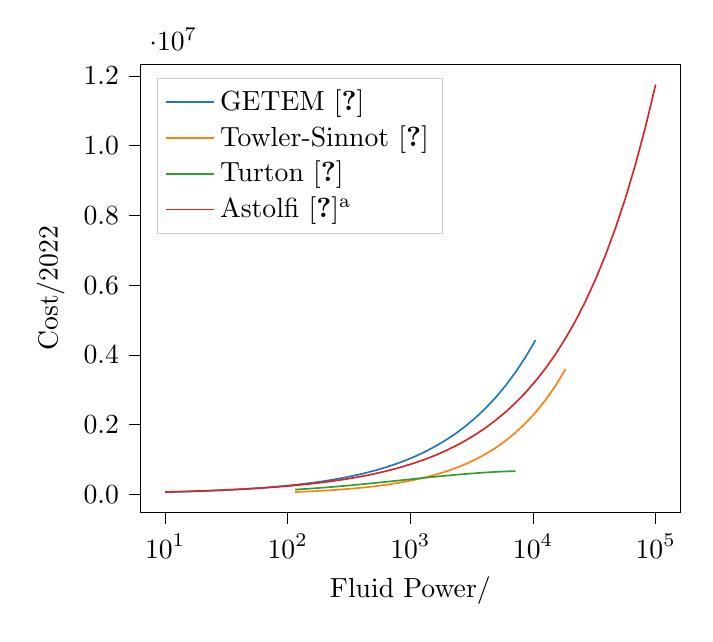
\begin{tikzpicture}

\definecolor{crimson2143940}{RGB}{214,39,40}
\definecolor{darkgray176}{RGB}{176,176,176}
\definecolor{darkorange25512714}{RGB}{255,127,14}
\definecolor{forestgreen4416044}{RGB}{44,160,44}
\definecolor{lightgray204}{RGB}{204,204,204}
\definecolor{steelblue31119180}{RGB}{31,119,180}

\begin{axis}[
legend cell align={left},
legend style={
  fill opacity=0.8,
  draw opacity=1,
  text opacity=1,
  at={(0.03,0.97)},
  anchor=north west,
  draw=lightgray204
},
log basis x={10},
tick align=outside,
tick pos=left,
unbounded coords=jump,
x grid style={darkgray176},
xlabel={Fluid Power/\unit{\kilo\watt}},
xmin=6.30957344480193, xmax=158489.319246111,
xmode=log,
xtick style={color=black},
xtick={0.1,1,10,100,1000,10000,100000,1000000,10000000},
xticklabels={
  \(\displaystyle {10^{-1}}\),
  \(\displaystyle {10^{0}}\),
  \(\displaystyle {10^{1}}\),
  \(\displaystyle {10^{2}}\),
  \(\displaystyle {10^{3}}\),
  \(\displaystyle {10^{4}}\),
  \(\displaystyle {10^{5}}\),
  \(\displaystyle {10^{6}}\),
  \(\displaystyle {10^{7}}\)
},
y grid style={darkgray176},
ylabel={Cost/\unit{\USD}2022},
ymin=-524986.649421086, ymax=12340066.2524408,
ytick style={color=black},
ytick={-2000000,0,2000000,4000000,6000000,8000000,10000000,12000000,14000000},
yticklabels={\ensuremath{-}0.2,0.0,0.2,0.4,0.6,0.8,1.0,1.2,1.4}
]
\addplot [semithick, steelblue31119180]
table {%
10 59788.4824817265
12.0679264063933 67123.0393006052
14.5634847750124 75359.6324932257
17.5751062485479 84609.4948622484
21.2095088792019 94997.6142710276
25.5954792269954 106664.439612931
30.8884359647748 119767.799013301
37.2759372031494 134485.05675104
44.9843266896944 151015.538703222
54.2867543932386 169583.259849204
65.5128556859551 190439.991572964
79.060432109077 213868.711232913
95.4095476349994 240187.481793977
115.139539932645 269753.815312304
138.949549437314 302969.580813195
167.683293681101 340286.524703028
202.358964772516 382212.480413484
244.205309454865 429318.353612282
294.705170255181 482245.980165192
355.648030622313 541716.966253057
429.193426012878 608542.633807993
517.947467923121 683635.209930004
625.055192527397 768020.416398915
754.312006335462 862851.635054618
910.298177991522 969425.8469605
1098.54114198756 1089201.56820559
1325.71136559011 1223819.03329524
1599.85871960606 1375122.90872839
1930.69772888325 1545187.85501252
2329.95181051537 1736347.29553391
2811.76869797423 1951225.79595447
3393.22177189533 2192775.50879269
4094.91506238042 2464317.19529524
4941.71336132383 2769586.40143816
5963.62331659464 3112785.43783989
7196.85673001151 3498641.89556677
8685.11373751352 3932474.52244453
10481.1313415469 4420267.38888457
12648.552168553 nan
15264.1796717523 nan
18420.6996932672 nan
22229.9648252619 nan
26826.9579527973 nan
32374.5754281764 nan
39069.3993705461 nan
47148.6636345739 nan
56898.6602901829 nan
68664.88450043 nan
82864.2772854684 nan
100000 nan
};
\addlegendentry{GETEM \cite{GETEM2016}}
\addplot [semithick, darkorange25512714]
table {%
10 nan
12.0679264063933 nan
14.5634847750124 nan
17.5751062485479 nan
21.2095088792019 nan
25.5954792269954 nan
30.8884359647748 nan
37.2759372031494 nan
44.9843266896944 nan
54.2867543932386 nan
65.5128556859551 nan
79.060432109077 nan
95.4095476349994 nan
115.139539932645 63335.4835020017
138.949549437314 75467.4169450851
167.683293681101 89436.0692963859
202.358964772516 105519.511348464
244.205309454865 124037.912532561
294.705170255181 145359.914458811
355.648030622313 169909.969381125
429.193426012878 198176.789671889
517.947467923121 230723.076508262
625.055192527397 268196.721436821
754.312006335462 311343.703803557
910.298177991522 361022.940795436
1098.54114198756 418223.385709934
1325.71136559011 484083.714823912
1599.85871960606 559914.994763872
1930.69772888325 647226.781611778
2329.95181051537 747757.171295429
2811.76869797423 863507.399469679
3393.22177189533 996781.679660497
4094.91506238042 1150233.07272075
4941.71336132383 1326916.30071056
5963.62331659464 1530348.55655617
7196.85673001151 1764579.52001141
8685.11373751352 2034271.97371357
10481.1313415469 2344794.6241393
12648.552168553 2702328.97522614
15264.1796717523 3113992.38216869
18420.6996932672 3587979.73499341
22229.9648252619 nan
26826.9579527973 nan
32374.5754281764 nan
39069.3993705461 nan
47148.6636345739 nan
56898.6602901829 nan
68664.88450043 nan
82864.2772854684 nan
100000 nan
};
\addlegendentry{Towler-Sinnot \cite{TowlerGavin2013}}
\addplot [semithick, forestgreen4416044]
table {%
10 nan
12.0679264063933 nan
14.5634847750124 nan
17.5751062485479 nan
21.2095088792019 nan
25.5954792269954 nan
30.8884359647748 nan
37.2759372031494 nan
44.9843266896944 nan
54.2867543932386 nan
65.5128556859551 nan
79.060432109077 nan
95.4095476349994 nan
115.139539932645 133245.078454807
138.949549437314 151787.240953468
167.683293681101 171969.862119461
202.358964772516 193777.079213165
244.205309454865 217162.810822553
294.705170255181 242047.994847198
355.648030622313 268318.433946475
429.193426012878 295823.395729513
517.947467923121 324375.101986061
625.055192527397 353749.220660979
754.312006335462 383686.446270814
910.298177991522 413895.219702568
1098.54114198756 444055.597926169
1325.71136559011 473824.239622109
1599.85871960606 502840.425973717
1930.69772888325 530732.989083496
2329.95181051537 557127.976002622
2811.76869797423 581656.836610475
3393.22177189533 603964.890842895
4094.91506238042 623719.807088959
4941.71336132383 640619.810612618
5963.62331659464 654401.3397526
7196.85673001151 664845.878952853
8685.11373751352 nan
10481.1313415469 nan
12648.552168553 nan
15264.1796717523 nan
18420.6996932672 nan
22229.9648252619 nan
26826.9579527973 nan
32374.5754281764 nan
39069.3993705461 nan
47148.6636345739 nan
56898.6602901829 nan
68664.88450043 nan
82864.2772854684 nan
100000 nan
};
\addlegendentry{Turton \cite{Turton2012}}
\addplot [semithick, crimson2143940]
table {%
10 64653.3163168255
12.0679264063933 71814.1758316322
14.5634847750124 79770.9519022951
17.5751062485479 88612.4781483075
21.2095088792019 98437.5515828551
25.5954792269954 109356.056440862
30.8884359647748 121490.215598201
37.2759372031494 134975.984175167
44.9843266896944 149964.601600174
54.2867543932386 166624.320288395
65.5128556859551 185142.331187596
79.060432109077 205726.908785633
95.4095476349994 228609.800789613
115.139539932645 254048.890607977
138.949549437314 282331.164029648
167.683293681101 313776.015139448
202.358964772516 348738.930581275
244.205309454865 387615.595830742
294.705170255181 430846.472223774
355.648030622313 478921.899170401
429.193426012878 532387.782334881
517.947467923121 591851.935663786
625.055192527397 657991.153082109
754.312006335462 731559.094553557
910.298177991522 813395.081127094
1098.54114198756 904433.90469284
1325.71136559011 1005716.77058728
1599.85871960606 1118403.50507804
1930.69772888325 1243786.17529902
2329.95181051537 1383304.28659539
2811.76869797423 1538561.74169731
3393.22177189533 1711345.7679206
4094.91506238042 1903648.04297058
4941.71336132383 2117688.277217
5963.62331659464 2355940.54086408
7196.85673001151 2621162.6586551
8685.11373751352 2916429.03306967
10481.1313415469 3245167.29988993
12648.552168553 3611199.26808874
15264.1796717523 4018786.64985402
18420.6996932672 4472682.14691443
22229.9648252619 4978186.52695965
26826.9579527973 5541212.39974543
32374.5754281764 6168355.48743119
39069.3993705461 6866974.27894149
47148.6636345739 7645279.06492523
56898.6602901829 8512431.4696264
68664.88450043 9478655.73026279
82864.2772854684 10555363.1251224
100000 11755291.120538
};
\addlegendentry{Astolfi \cite{Astolfi2014B}\textsuperscript{a}}
\end{axis}

\end{tikzpicture}
